

\section{Evaluating Keyphrase Recognition Performance}
\label{sec:recognition_evaluation}

In this section, I present performance results for the ensemble of classification models learnt from keyphrase data.
 The model is organized as follows:

\begin{itemize}
\item An individiual classification model is learnt for every keyphrase apart from "random talk".
 The objective of the classification is to distinguish between the true keyphrase and "random talk".
\item For a test audio clip, all 8 classification models are used to get class probabilities for the associated keyphrase.
 The keyphrase with the maximum class probability is chosen and compared to a confidence threshold.
 If the class probability is greater or equal to than the confidence threshold, the classification output is the true keyphrase.
 If the class probability is lower than the confidence threshold, the classification output is "random talk".
\end{itemize}


Summarized in \cref{tab:probs_raw_audio,tab:probs_raw_audio_hamming_1,tab:probs_raw_audio_hamming_4,tab:probs_raw_audio_hamming_16,tab:probs_samplerate_2000,tab:probs_samplerate_1000,tab:probs_samplerate_2000_hamming_1,tab:probs_samplerate_1000_hamming_1,tab:probs_samplerate_2000_hamming_4,tab:probs_samplerate_1000_hamming_4,tab:probs_samplerate_2000_hamming_16,tab:probs_precision_1_hamming_1,tab:probs_precision_1_hamming_4,tab:probs_precision_1_hamming_16}
 are the mean class probabilities for different keyphrase audio examples using different keyphrase models.
 Each table corresponds to a different obfuscation technique, as noted in the caption.
 Each table corresponds to a different obfuscation technique.
 Each row corresponds to a classification model for a single keyphrase.
 Each column corresponds to audio examples for a single keyphrase, or audio examples for "random talk".
 The class probabilities in the table indicate the level to which the model has learnt the training set.


Examples for "random talk" are an assortment of choices from three sources:
\begin{itemize}
\item TED-LIUM Speech Corpus
\item Babble Noise Examples (Cafeteria noise, Public Transit Vehicle Noise)
\item "random talk" examples from the \texttt{dbHound Keyphrase}\footnote{The \texttt{dbHound Keyphrase} android application can be found on the Google Play Store at \url{https://play.google.com/store/apps/details?id=edu.wisc.cs.dbhound}.} android application
\end{itemize}

Figures \ref{fig:roc_raw_audio} \ref{fig:roc_samplerate} \ref{fig:roc_precision_bits} show the Receiver Operating Curves (ROC) for different obfuscation techniques.
 The Receiver Operating Curve shows the variation of the false positive ratio and true positive ratio when the confidence threshold for classification is varied.
 These curves help understand how well the model is likely to perform in real life.


\begin{table}[!th]
\begin{tabular}{cccccccccc}%
\hline%
None&\rotate{random talk}{70}&\rotate{okay google}{70}&\rotate{hey siri}{70}&\rotate{hey cortana}{70}&\rotate{nine one one}{70}&\rotate{call mom}{70}&\rotate{take a picture}{70}&\rotate{play a song}{70}&\rotate{make a note}{70}\\%
\hline%
okay google&0.01&\textbf{0.83}&0.01&0.01&0.0&0.0&0.01&0.0&0.01\\%
hey siri&0.01&0.05&\textbf{0.64}&0.01&0.0&0.0&0.09&0.03&0.02\\%
hey cortana&0.01&0.03&0.03&\textbf{0.66}&0.04&0.02&0.02&0.02&0.02\\%
nine one one&0.0&0.0&0.0&0.0&\textbf{0.83}&0.03&0.0&0.01&0.01\\%
call mom&0.01&0.0&0.01&0.06&0.03&\textbf{0.94}&0.0&0.05&0.0\\%
take a picture&0.01&0.02&0.03&0.01&0.0&0.0&\textbf{0.77}&0.0&0.01\\%
play a song&0.02&0.01&0.03&0.02&0.01&0.04&0.01&\textbf{0.71}&0.03\\%
make a note&0.02&0.03&0.02&0.02&0.01&0.03&0.03&0.01&\textbf{0.67}\\%
\hline%
\end{tabular}
\caption{Mean Class Probabilities from 350 audio examples. Each row corresponds to a different keyphrase classification model. Each column corresponds to a different keyphrase audio example. \emph{Obfuscation technique: no obfuscation}}
\label{tab:probs_raw_audio}
\end{table}



\begin{table}[!th]
\begin{tabular}{cccccccccc}%
\hline%
None&\rotate{random talk}{70}&\rotate{okay google}{70}&\rotate{hey siri}{70}&\rotate{hey cortana}{70}&\rotate{nine one one}{70}&\rotate{call mom}{70}&\rotate{take a picture}{70}&\rotate{play a song}{70}&\rotate{make a note}{70}\\%
\hline%
okay google&0.07&\textbf{0.52}&0.06&0.12&0.09&0.1&0.08&0.08&0.1\\%
hey siri&0.1&0.14&\textbf{0.53}&0.14&0.12&0.09&0.14&0.13&0.11\\%
hey cortana&0.06&0.09&0.08&\textbf{0.58}&0.07&0.08&0.11&0.08&0.11\\%
nine one one&0.02&0.04&0.04&0.03&\textbf{0.77}&0.12&0.02&0.08&0.05\\%
call mom&0.01&0.01&0.03&0.04&0.05&\textbf{0.83}&0.02&0.1&0.06\\%
take a picture&0.01&0.05&0.03&0.07&0.06&0.03&\textbf{0.38}&0.09&0.05\\%
play a song&0.0&0.01&0.01&0.03&0.03&0.05&0.01&\textbf{0.39}&0.02\\%
make a note&0.04&0.06&0.08&0.06&0.1&0.08&0.05&0.08&\textbf{0.44}\\%
\hline%
\end{tabular}
\caption{Mean Class Probabilities from 350 audio examples. Each row corresponds to a different keyphrase classification model. Each column corresponds to a different keyphrase audio example. \emph{Obfuscation technique: hamming reduction on every 1 sample}}
\label{tab:probs_raw_audio_hamming_1}
\end{table}





\begin{table}[!th]
\begin{tabular}{cccccccccc}%
\hline%
None&\rotate{random talk}{70}&\rotate{okay google}{70}&\rotate{hey siri}{70}&\rotate{hey cortana}{70}&\rotate{nine one one}{70}&\rotate{call mom}{70}&\rotate{take a picture}{70}&\rotate{play a song}{70}&\rotate{make a note}{70}\\%
\hline%
okay google&0.04&\textbf{0.79}&0.06&0.12&0.03&0.03&0.07&0.05&0.05\\%
hey siri&0.06&0.07&\textbf{0.45}&0.08&0.04&0.05&0.07&0.04&0.05\\%
hey cortana&0.01&0.07&0.04&\textbf{0.57}&0.01&0.02&0.08&0.03&0.05\\%
nine one one&0.02&0.03&0.04&0.03&\textbf{0.64}&0.15&0.02&0.07&0.03\\%
call mom&0.0&0.0&0.02&0.02&0.05&\textbf{0.71}&0.01&0.05&0.05\\%
take a picture&0.03&0.05&0.02&0.05&0.01&0.01&\textbf{0.63}&0.02&0.02\\%
play a song&0.04&0.05&0.07&0.06&0.13&0.1&0.06&\textbf{0.32}&0.09\\%
make a note&0.0&0.01&0.01&0.02&0.02&0.03&0.02&0.04&\textbf{0.52}\\%
\hline%
\end{tabular}
\caption{Mean Class Probabilities from 350 audio examples. Each row corresponds to a different keyphrase classification model. Each column corresponds to a different keyphrase audio example. \emph{Obfuscation technique: hamming reduction on every 4 samples}}
\label{tab:probs_raw_audio_hamming_4}
\end{table}





\begin{table}[!th]
\begin{tabular}{cccccccccc}%
\hline%
None&\rotate{random talk}{70}&\rotate{okay google}{70}&\rotate{hey siri}{70}&\rotate{hey cortana}{70}&\rotate{nine one one}{70}&\rotate{call mom}{70}&\rotate{take a picture}{70}&\rotate{play a song}{70}&\rotate{make a note}{70}\\%
\hline%
okay google&0.03&\textbf{0.85}&0.0&0.09&0.0&0.0&0.01&0.0&0.0\\%
hey siri&0.0&0.0&\textbf{0.99}&0.0&0.0&0.0&0.0&0.0&0.0\\%
hey cortana&0.01&0.02&0.02&\textbf{0.91}&0.01&0.01&0.0&0.02&0.03\\%
nine one one&0.01&0.0&0.0&0.01&\textbf{0.98}&0.0&0.0&0.01&0.0\\%
call mom&0.0&0.0&0.01&0.0&0.0&\textbf{0.81}&0.0&0.01&0.0\\%
take a picture&0.0&0.0&0.0&0.0&0.0&0.0&\textbf{0.7}&0.0&0.0\\%
play a song&0.0&0.0&0.0&0.01&0.01&0.01&0.0&\textbf{0.68}&0.0\\%
make a note&0.02&0.0&0.0&0.0&0.0&0.0&0.0&0.0&\textbf{0.87}\\%
\hline%
\end{tabular}
\caption{Mean Class Probabilities from 350 audio examples. Each row corresponds to a different keyphrase classification model. Each column corresponds to a different keyphrase audio example. \emph{Obfuscation technique: hamming reduction on every 16 samples}}
\label{tab:probs_raw_audio_hamming_16}
\end{table}



\clearpage


\begin{table}[!th]
\begin{tabular}{cccccccccc}%
\hline%
None&\rotate{random talk}{70}&\rotate{okay google}{70}&\rotate{hey siri}{70}&\rotate{hey cortana}{70}&\rotate{nine one one}{70}&\rotate{call mom}{70}&\rotate{take a picture}{70}&\rotate{play a song}{70}&\rotate{make a note}{70}\\%
\hline%
okay google&0.03&\textbf{0.73}&0.03&0.02&0.01&0.0&0.05&0.01&0.02\\%
hey siri&0.01&0.03&\textbf{0.51}&0.03&0.01&0.02&0.05&0.02&0.03\\%
hey cortana&0.02&0.05&0.03&\textbf{0.74}&0.02&0.02&0.05&0.03&0.01\\%
nine one one&0.04&0.03&0.02&0.07&\textbf{0.87}&0.04&0.03&0.03&0.02\\%
call mom&0.0&0.0&0.02&0.02&0.04&\textbf{0.92}&0.0&0.08&0.02\\%
take a picture&0.02&0.02&0.04&0.01&0.0&0.0&\textbf{0.49}&0.01&0.01\\%
play a song&0.01&0.01&0.1&0.04&0.03&0.13&0.01&\textbf{0.81}&0.04\\%
make a note&0.04&0.06&0.03&0.03&0.04&0.03&0.02&0.04&\textbf{0.58}\\%
\hline%
\end{tabular}
\caption{Mean Class Probabilities from 350 audio examples. Each row corresponds to a different keyphrase classification model. Each column corresponds to a different keyphrase audio example. \emph{Obfuscation technique: samplerate reduced to 2000 Hz}}
\label{tab:probs_samplerate_2000}
\end{table}







\begin{table}[!th]
\begin{tabular}{cccccccccc}%
\hline%
None&\rotate{random talk}{70}&\rotate{okay google}{70}&\rotate{hey siri}{70}&\rotate{hey cortana}{70}&\rotate{nine one one}{70}&\rotate{call mom}{70}&\rotate{take a picture}{70}&\rotate{play a song}{70}&\rotate{make a note}{70}\\%
\hline%
okay google&0.01&\textbf{0.34}&0.01&0.03&0.01&0.01&0.02&0.01&0.03\\%
hey siri&0.06&0.06&\textbf{0.06}&0.06&0.06&0.06&0.06&0.06&0.06\\%
hey cortana&0.01&0.04&0.07&\textbf{0.68}&0.03&0.01&0.03&0.08&0.04\\%
nine one one&0.01&0.01&0.02&0.01&\textbf{0.64}&0.02&0.02&0.02&0.01\\%
call mom&0.01&0.02&0.02&0.06&0.04&\textbf{0.62}&0.01&0.03&0.02\\%
take a picture&0.05&0.05&0.05&0.05&0.05&0.05&\textbf{0.05}&0.05&0.05\\%
play a song&0.04&0.05&0.11&0.03&0.09&0.11&0.03&\textbf{0.66}&0.06\\%
make a note&0.02&0.04&0.03&0.08&0.03&0.02&0.06&0.06&\textbf{0.26}\\%
\hline%
\end{tabular}
\caption{Mean Class Probabilities from 350 audio examples. Each row corresponds to a different keyphrase classification model. Each column corresponds to a different keyphrase audio example. \emph{Obfuscation technique: samplerate reduced to 1000 Hz}}
\label{tab:probs_samplerate_1000}
\end{table}





\begin{table}[!th]
\begin{tabular}{cccccccccc}%
\hline%
None&\rotate{random talk}{70}&\rotate{okay google}{70}&\rotate{hey siri}{70}&\rotate{hey cortana}{70}&\rotate{nine one one}{70}&\rotate{call mom}{70}&\rotate{take a picture}{70}&\rotate{play a song}{70}&\rotate{make a note}{70}\\%
\hline%
okay google&0.03&\textbf{0.49}&0.05&0.06&0.03&0.02&0.04&0.02&0.02\\%
hey siri&0.07&0.07&\textbf{0.43}&0.1&0.1&0.1&0.09&0.1&0.07\\%
hey cortana&0.02&0.06&0.04&\textbf{0.44}&0.01&0.01&0.06&0.01&0.02\\%
nine one one&0.03&0.04&0.05&0.04&\textbf{0.72}&0.16&0.02&0.09&0.04\\%
call mom&0.01&0.0&0.02&0.02&0.03&\textbf{0.55}&0.02&0.04&0.06\\%
take a picture&0.06&0.05&0.04&0.06&0.01&0.01&\textbf{0.63}&0.03&0.02\\%
play a song&0.01&0.0&0.01&0.01&0.05&0.07&0.01&\textbf{0.43}&0.05\\%
make a note&0.01&0.03&0.04&0.05&0.04&0.07&0.04&0.04&\textbf{0.42}\\%
\hline%
\end{tabular}
\caption{Mean Class Probabilities from 350 audio examples. Each row corresponds to a different keyphrase classification model. Each column corresponds to a different keyphrase audio example. \emph{Obfuscation technique: samplerate reduced to 2000 Hz followed by hamming reduction on every 1 sample}}
\label{tab:probs_samplerate_2000_hamming_1}
\end{table}








\begin{table}[!th]
\begin{tabular}{cccccccccc}%
\hline%
None&\rotate{random talk}{70}&\rotate{okay google}{70}&\rotate{hey siri}{70}&\rotate{hey cortana}{70}&\rotate{nine one one}{70}&\rotate{call mom}{70}&\rotate{take a picture}{70}&\rotate{play a song}{70}&\rotate{make a note}{70}\\%
\hline%
okay google&0.05&\textbf{0.86}&0.03&0.09&0.03&0.05&0.03&0.04&0.03\\%
hey siri&0.03&0.01&\textbf{0.96}&0.03&0.03&0.02&0.04&0.01&0.06\\%
hey cortana&0.01&0.01&0.01&\textbf{0.51}&0.01&0.01&0.01&0.01&0.01\\%
nine one one&0.0&0.0&0.0&0.0&\textbf{1.0}&0.0&0.0&0.0&0.0\\%
call mom&0.01&0.0&0.01&0.0&0.0&\textbf{0.99}&0.0&0.01&0.0\\%
take a picture&0.01&0.05&0.01&0.03&0.01&0.02&\textbf{0.87}&0.01&0.03\\%
play a song&0.02&0.0&0.0&0.0&0.03&0.0&0.01&\textbf{0.9}&0.0\\%
make a note&0.0&0.0&0.0&0.0&0.0&0.0&0.0&0.0&\textbf{1.0}\\%
\hline%
\end{tabular}
\caption{Mean Class Probabilities from 350 audio examples. Each row corresponds to a different keyphrase classification model. Each column corresponds to a different keyphrase audio example. \emph{Obfuscation technique: samplerate reduced to 1000 Hz followed by hamming reduction on every 1 sample}}
\label{tab:probs_samplerate_1000_hamming_1}
\end{table}









\begin{table}[!th]
\begin{tabular}{cccccccccc}%
\hline%
None&\rotate{random talk}{70}&\rotate{okay google}{70}&\rotate{hey siri}{70}&\rotate{hey cortana}{70}&\rotate{nine one one}{70}&\rotate{call mom}{70}&\rotate{take a picture}{70}&\rotate{play a song}{70}&\rotate{make a note}{70}\\%
\hline%
okay google&0.01&\textbf{0.84}&0.01&0.01&0.02&0.01&0.01&0.02&0.01\\%
hey siri&0.0&0.0&\textbf{0.99}&0.0&0.0&0.0&0.0&0.0&0.0\\%
hey cortana&0.04&0.04&0.06&\textbf{0.78}&0.01&0.0&0.04&0.02&0.03\\%
nine one one&0.01&0.0&0.0&0.04&\textbf{0.91}&0.0&0.01&0.02&0.01\\%
call mom&0.0&0.0&0.0&0.0&0.0&\textbf{0.28}&0.0&0.0&0.0\\%
take a picture&0.0&0.0&0.0&0.0&0.0&0.0&\textbf{1.0}&0.0&0.0\\%
play a song&0.01&0.0&0.0&0.0&0.0&0.0&0.0&\textbf{0.98}&0.0\\%
make a note&0.02&0.0&0.01&0.0&0.01&0.03&0.01&0.03&\textbf{0.86}\\%
\hline%
\end{tabular}
\caption{Mean Class Probabilities from 350 audio examples. Each row corresponds to a different keyphrase classification model. Each column corresponds to a different keyphrase audio example. \emph{Obfuscation technique: samplerate reduced to 2000 Hz followed by hamming reduction on every 4 samples}}
\label{tab:probs_samplerate_2000_hamming_4}
\end{table}







\begin{table}[!th]
\begin{tabular}{cccccccccc}%
\hline%
None&\rotate{random talk}{70}&\rotate{okay google}{70}&\rotate{hey siri}{70}&\rotate{hey cortana}{70}&\rotate{nine one one}{70}&\rotate{call mom}{70}&\rotate{take a picture}{70}&\rotate{play a song}{70}&\rotate{make a note}{70}\\%
\hline%
okay google&0.0&\textbf{0.48}&0.0&0.01&0.0&0.0&0.0&0.01&0.0\\%
hey siri&0.03&0.03&\textbf{0.72}&0.02&0.03&0.02&0.08&0.01&0.02\\%
hey cortana&0.02&0.06&0.04&\textbf{0.77}&0.03&0.03&0.01&0.03&0.11\\%
nine one one&0.02&0.02&0.01&0.01&\textbf{0.82}&0.04&0.01&0.01&0.01\\%
call mom&0.01&0.02&0.02&0.01&0.03&\textbf{0.1}&0.02&0.03&0.01\\%
take a picture&0.03&0.02&0.01&0.01&0.01&0.03&\textbf{0.88}&0.01&0.01\\%
play a song&0.01&0.05&0.03&0.02&0.06&0.05&0.01&\textbf{0.92}&0.02\\%
make a note&0.01&0.04&0.04&0.02&0.01&0.01&0.0&0.01&\textbf{0.73}\\%
\hline%
\end{tabular}
\caption{Mean Class Probabilities from 350 audio examples. Each row corresponds to a different keyphrase classification model. Each column corresponds to a different keyphrase audio example. \emph{Obfuscation technique: samplerate reduced to 1000 Hz followed by hamming reduction every 4 samples}}
\label{tab:probs_samplerate_1000_hamming_4}
\end{table}








\begin{table}[!th]
\begin{tabular}{cccccccccc}%
\hline%
None&\rotate{random talk}{70}&\rotate{okay google}{70}&\rotate{hey siri}{70}&\rotate{hey cortana}{70}&\rotate{nine one one}{70}&\rotate{call mom}{70}&\rotate{take a picture}{70}&\rotate{play a song}{70}&\rotate{make a note}{70}\\%
\hline%
okay google&0.02&\textbf{0.72}&0.02&0.06&0.06&0.01&0.06&0.08&0.04\\%
hey siri&0.01&0.05&\textbf{0.11}&0.05&0.06&0.1&0.04&0.06&0.08\\%
hey cortana&0.02&0.02&0.01&\textbf{0.99}&0.01&0.0&0.01&0.02&0.01\\%
nine one one&0.04&0.05&0.07&0.07&\textbf{0.73}&0.12&0.05&0.09&0.08\\%
call mom&0.0&0.01&0.02&0.0&0.02&\textbf{0.85}&0.0&0.09&0.04\\%
take a picture&0.0&0.0&0.0&0.0&0.0&0.0&\textbf{1.0}&0.0&0.0\\%
play a song&0.01&0.0&0.0&0.0&0.0&0.0&0.0&\textbf{0.98}&0.0\\%
make a note&0.01&0.0&0.0&0.0&0.0&0.0&0.0&0.0&\textbf{1.0}\\%
\hline%
\end{tabular}
\caption{Mean Class Probabilities from 350 audio examples. Each row corresponds to a different keyphrase classification model. Each column corresponds to a different keyphrase audio example. \emph{Obfuscation technique: samplerate reduced to 2000 Hz followed by hamming reduction on every 16 samples}}
\label{tab:probs_samplerate_2000_hamming_16}
\end{table}




\begin{table}[!th]
\begin{tabular}{cccccccccc}%
\hline%
None&\rotate{random talk}{70}&\rotate{okay google}{70}&\rotate{hey siri}{70}&\rotate{hey cortana}{70}&\rotate{nine one one}{70}&\rotate{call mom}{70}&\rotate{take a picture}{70}&\rotate{play a song}{70}&\rotate{make a note}{70}\\%
\hline%
okay google&0.0&\textbf{1.0}&0.0&0.0&0.0&0.0&0.0&0.0&0.0\\%
hey siri&0.0&0.0&\textbf{0.76}&0.0&0.0&0.0&0.0&0.0&0.0\\%
hey cortana&0.01&0.0&0.0&\textbf{0.99}&0.0&0.0&0.0&0.0&0.01\\%
nine one one&0.0&0.0&0.0&0.0&\textbf{1.0}&0.0&0.0&0.0&0.0\\%
call mom&0.0&0.0&0.0&0.0&0.0&\textbf{1.0}&0.0&0.0&0.0\\%
take a picture&0.02&0.0&0.0&0.0&0.0&0.0&\textbf{1.0}&0.0&0.0\\%
play a song&0.0&0.0&0.0&0.0&0.0&0.0&0.0&\textbf{1.0}&0.0\\%
make a note&0.01&0.02&0.0&0.0&0.0&0.05&0.0&0.03&\textbf{0.95}\\%
\hline%
\end{tabular}
\caption{Mean Class Probabilities from 350 audio examples. Each row corresponds to a different keyphrase classification model. Each column corresponds to a different keyphrase audio example. \emph{Obfuscation technique: precision reduced to 1-bit}}
\label{tab:probs_precision_1_hamming_1}
\end{table}











\begin{table}[!th]
\begin{tabular}{cccccccccc}%
\hline%
None&\rotate{random talk}{70}&\rotate{okay google}{70}&\rotate{hey siri}{70}&\rotate{hey cortana}{70}&\rotate{nine one one}{70}&\rotate{call mom}{70}&\rotate{take a picture}{70}&\rotate{play a song}{70}&\rotate{make a note}{70}\\%
\hline%
okay google&0.03&\textbf{0.98}&0.0&0.01&0.0&0.0&0.01&0.0&0.0\\%
hey siri&0.01&0.02&\textbf{0.16}&0.03&0.02&0.02&0.03&0.02&0.02\\%
hey cortana&0.0&0.0&0.0&\textbf{1.0}&0.0&0.0&0.0&0.0&0.0\\%
nine one one&0.0&0.0&0.0&0.0&\textbf{0.9}&0.0&0.0&0.0&0.0\\%
call mom&0.04&0.06&0.06&0.07&0.06&\textbf{0.1}&0.07&0.07&0.06\\%
take a picture&0.05&0.04&0.04&0.04&0.05&0.06&\textbf{0.49}&0.06&0.05\\%
play a song&0.0&0.0&0.0&0.0&0.0&0.0&0.0&\textbf{1.0}&0.0\\%
make a note&0.0&0.0&0.0&0.0&0.0&0.0&0.0&0.0&\textbf{0.83}\\%
\hline%
\end{tabular}
\caption{Mean Class Probabilities from 350 audio examples. Each row corresponds to a different keyphrase classification model. Each column corresponds to a different keyphrase audio example. \emph{Obfuscation technique: precision reduced to 1-bit followed by hamming reduction on every 4 samples}}
\label{tab:probs_precision_1_hamming_4}
\end{table}



\begin{table}[!th]
\begin{tabular}{cccccccccc}%
\hline%
None&\rotate{random talk}{70}&\rotate{okay google}{70}&\rotate{hey siri}{70}&\rotate{hey cortana}{70}&\rotate{nine one one}{70}&\rotate{call mom}{70}&\rotate{take a picture}{70}&\rotate{play a song}{70}&\rotate{make a note}{70}\\%
\hline%
okay google&0.01&\textbf{0.79}&0.01&0.01&0.01&0.01&0.0&0.01&0.01\\%
hey siri&0.01&0.04&\textbf{0.84}&0.02&0.01&0.02&0.04&0.02&0.01\\%
hey cortana&0.02&0.02&0.03&\textbf{0.76}&0.04&0.03&0.03&0.03&0.03\\%
nine one one&0.01&0.06&0.03&0.01&\textbf{0.86}&0.03&0.0&0.02&0.06\\%
call mom&0.02&0.01&0.01&0.02&0.02&\textbf{0.64}&0.01&0.04&0.02\\%
take a picture&0.06&0.01&0.05&0.03&0.0&0.01&\textbf{0.7}&0.02&0.01\\%
play a song&0.08&0.05&0.04&0.08&0.04&0.12&0.05&\textbf{0.73}&0.06\\%
make a note&0.02&0.03&0.02&0.02&0.03&0.01&0.01&0.01&\textbf{0.68}\\%
\hline%
\end{tabular}
\caption{Mean Class Probabilities from 350 audio examples. Each row corresponds to a different keyphrase classification model. Each column corresponds to a different keyphrase audio example. \emph{Obfuscation technique: precision reduced to 1-bit followed by hamming reduction on every 16 samples}}
\label{tab:probs_precision_1_hamming_16}
\end{table}%


\clearpage


\begin{figure}[!th]
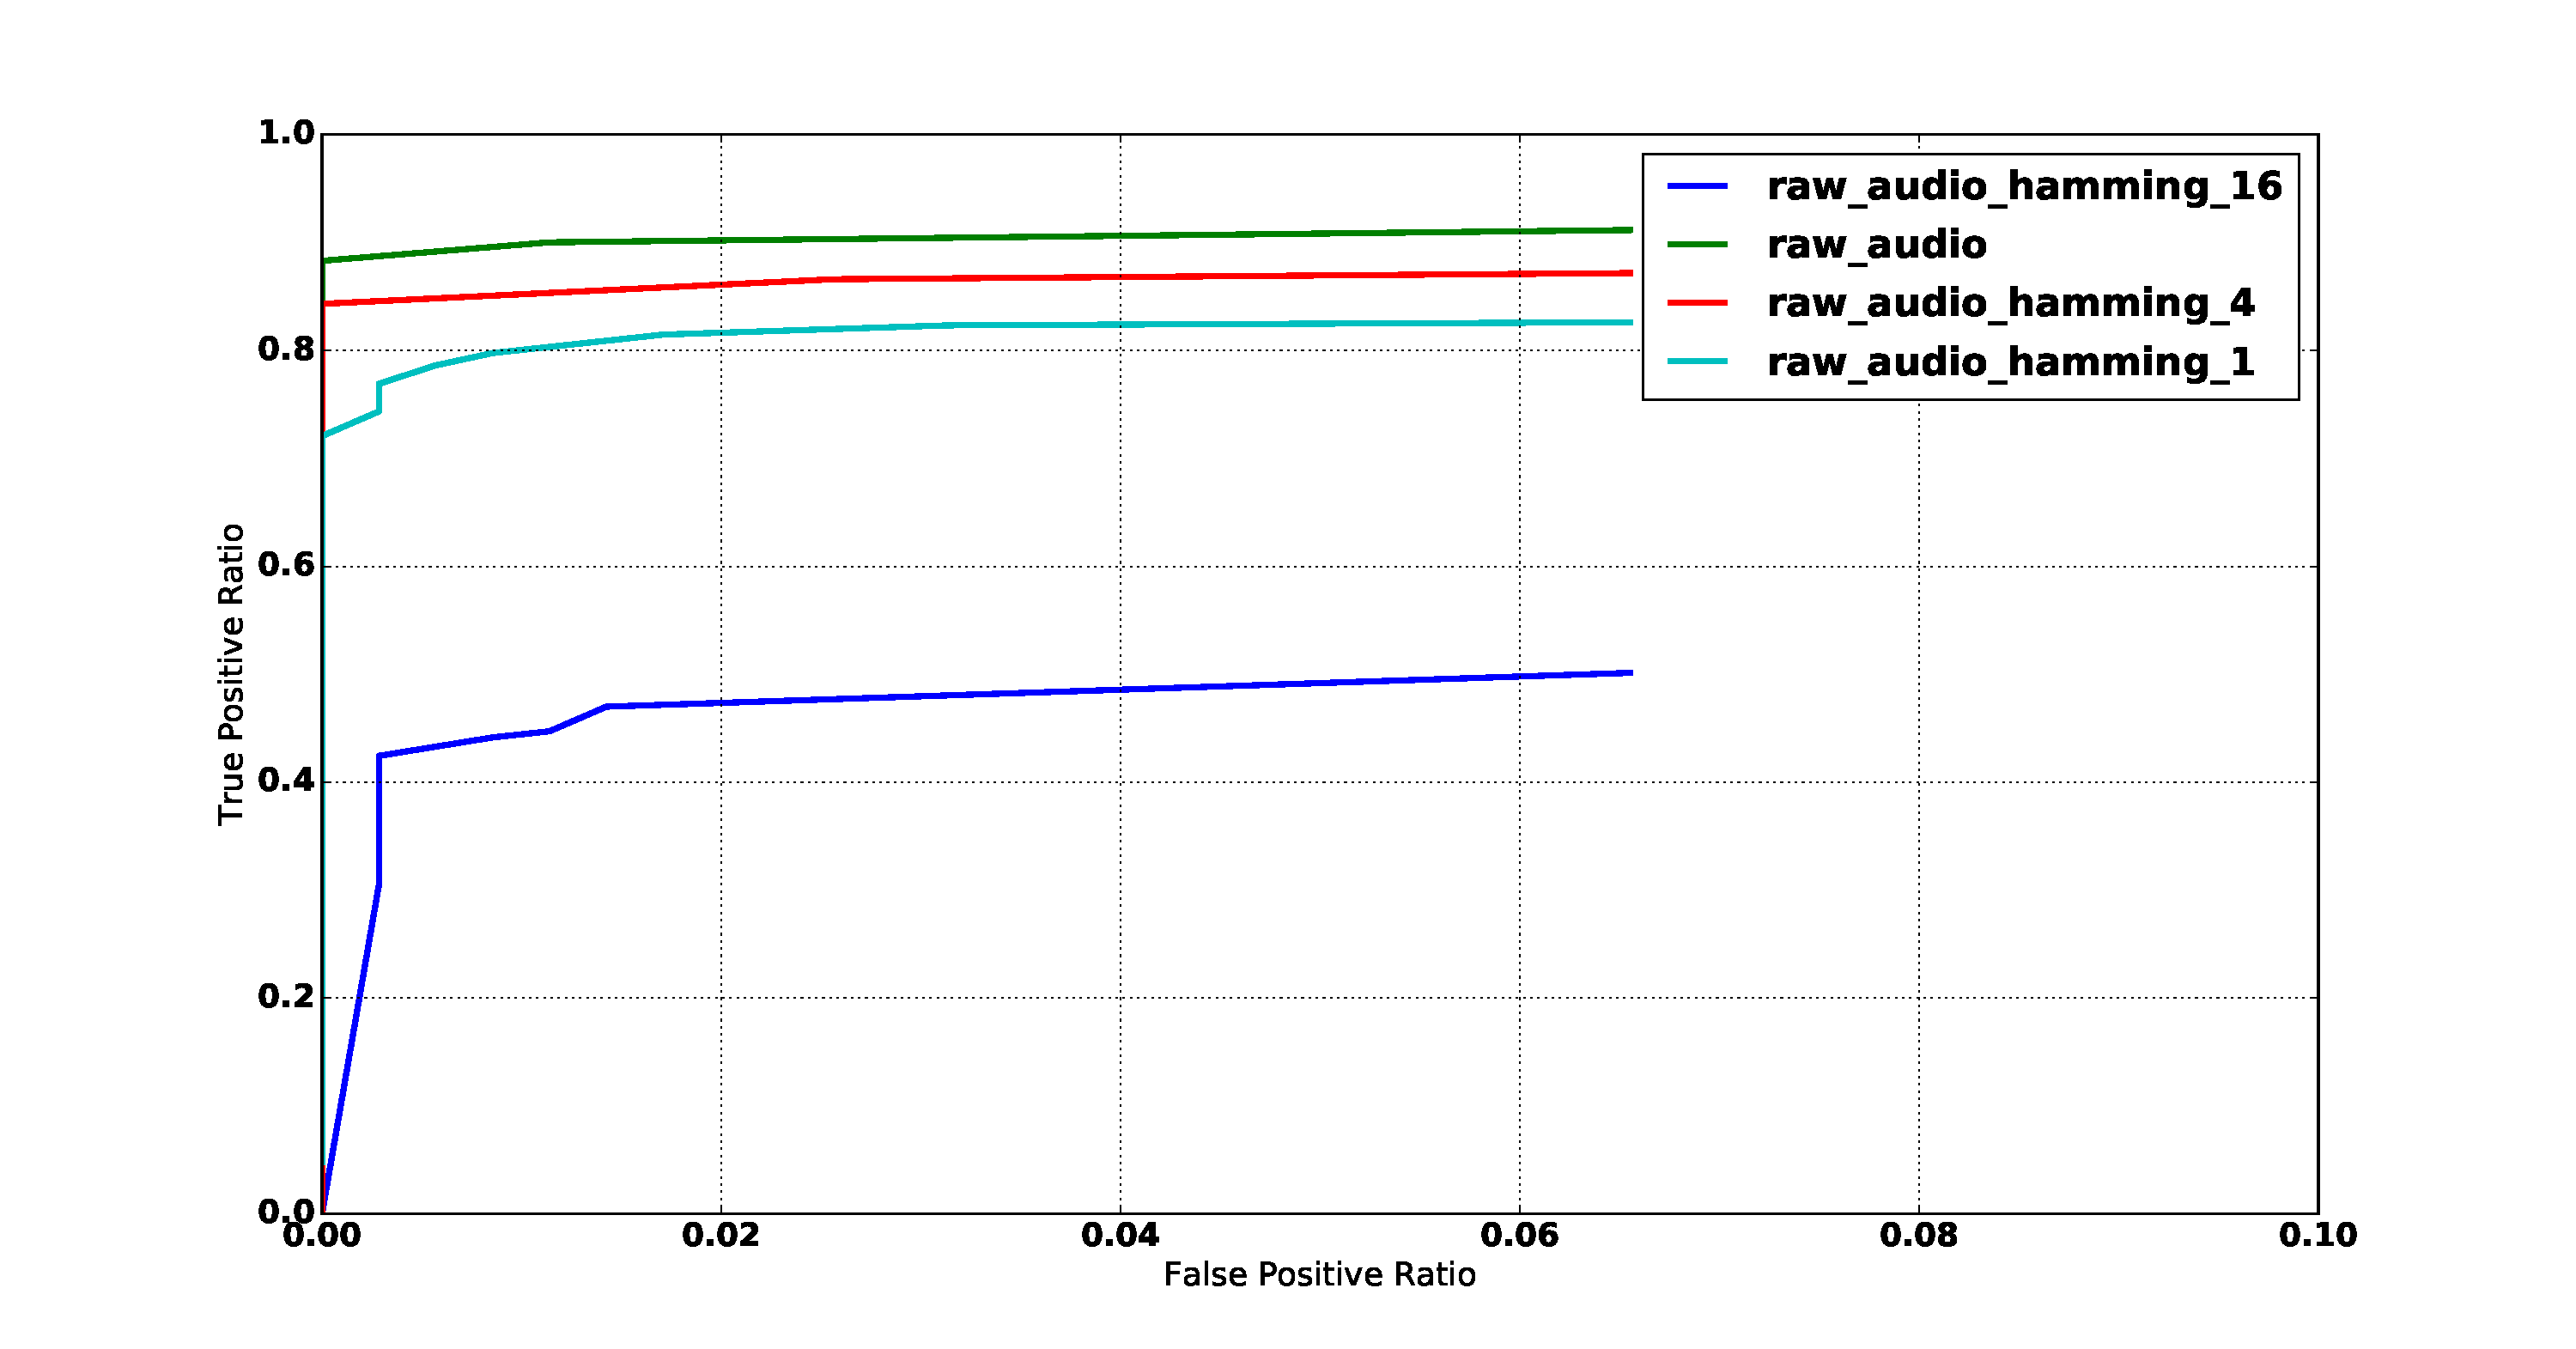
\includegraphics[width=\textwidth]{sound/roc_raw_audio.pdf}
\caption{Receiver Operating Curve (ROC) for Keyphrase Recognition on Raw Audio and Raw Audio obfuscated with Hamming Reduction}
\label{fig:roc_raw_audio}
\end{figure}



\begin{figure}[!th]
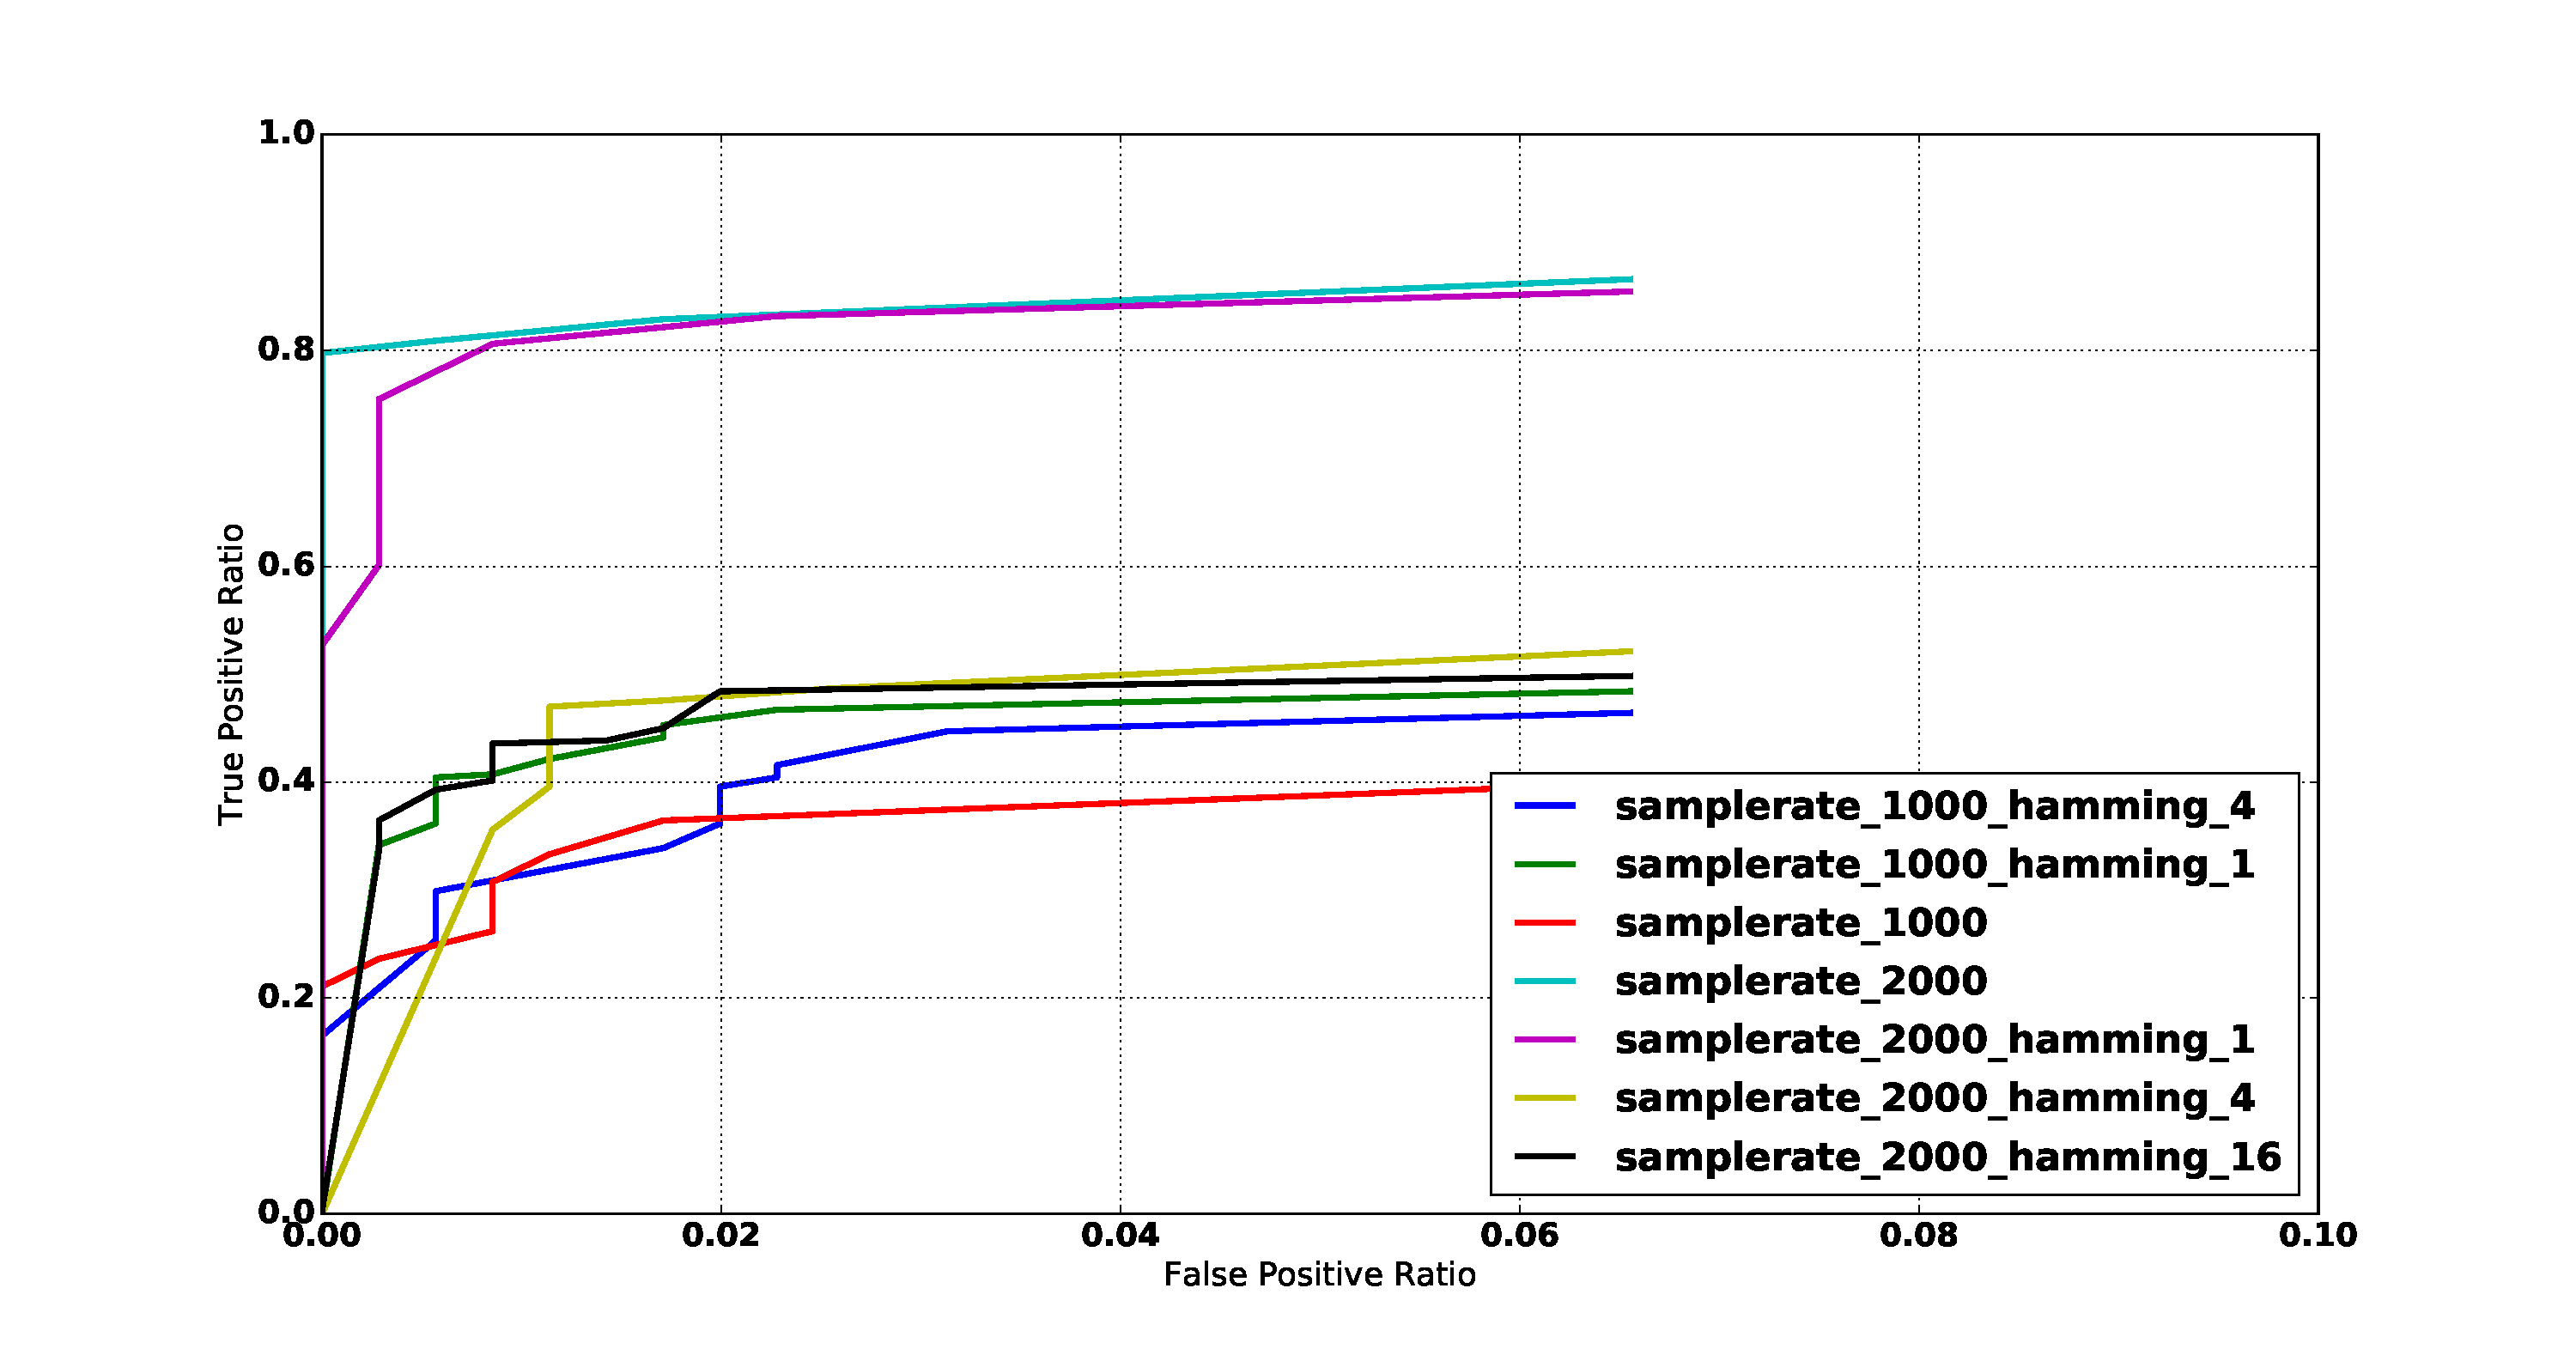
\includegraphics[width=\textwidth]{sound/roc_samplerate.pdf}
\caption{Receiver Operating Curve (ROC) for Keyphrase Recognition on Downsampled Audio and Downsampled Audio obfuscated with Hamming Reduction}
\label{fig:roc_samplerate}
\end{figure}



\begin{figure}[!th]
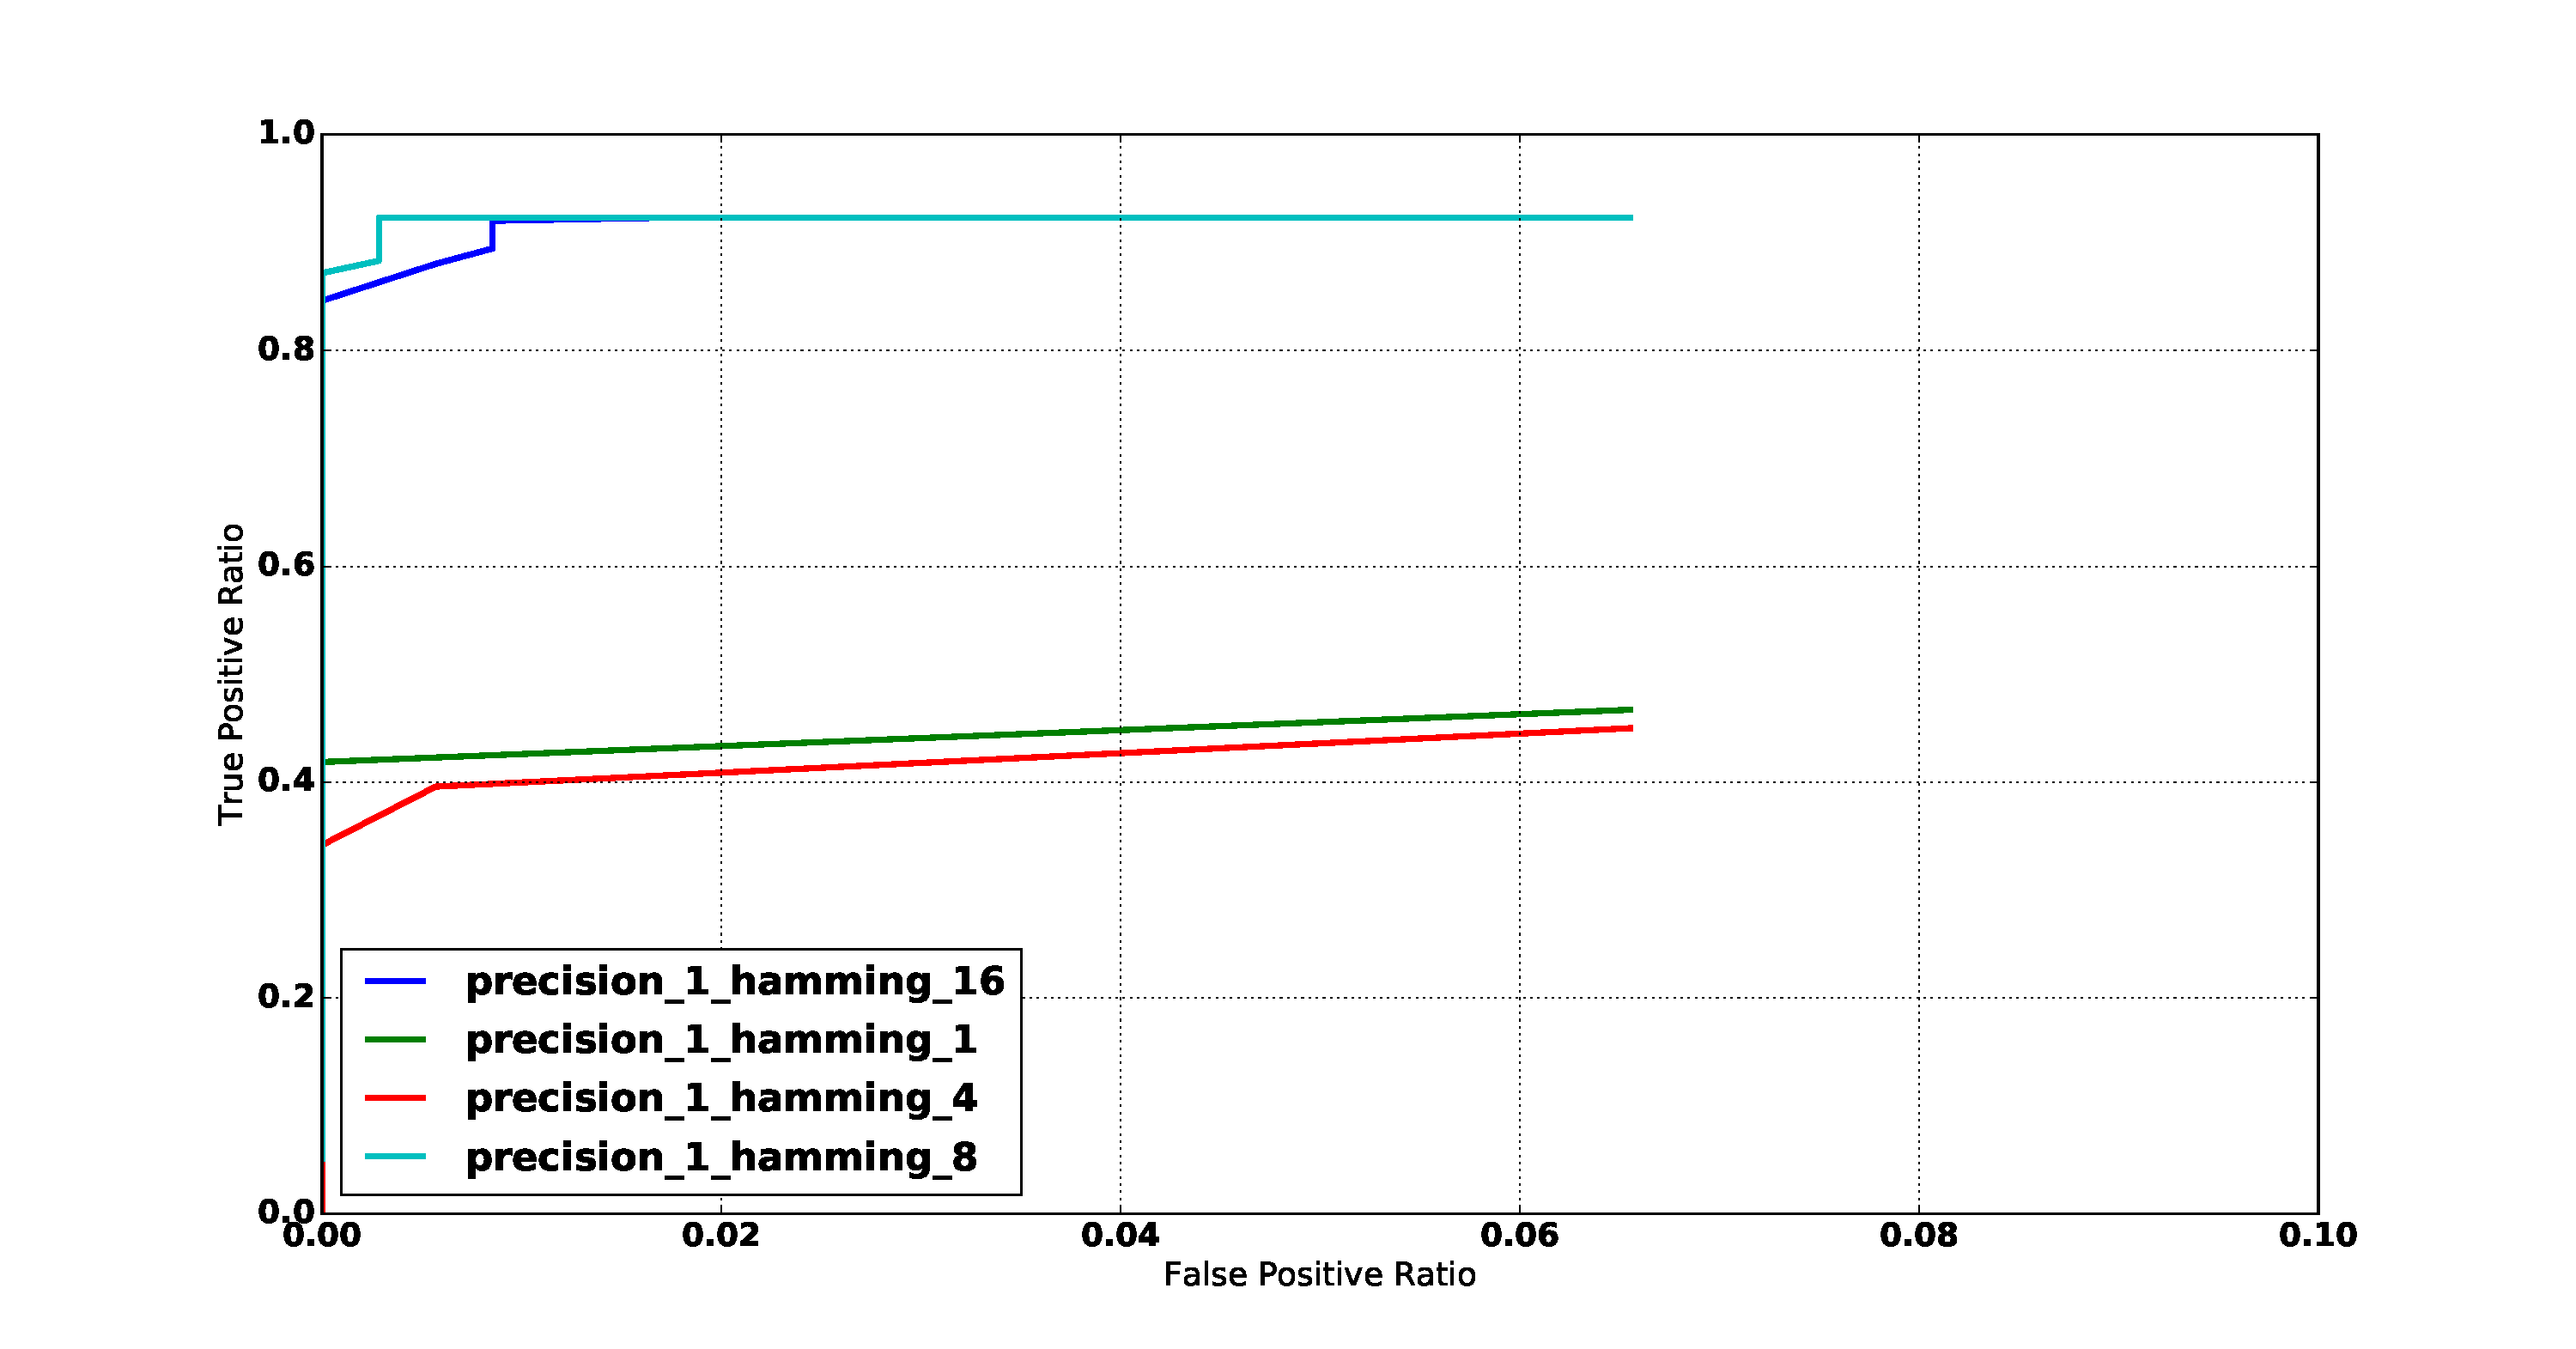
\includegraphics[width=\textwidth]{sound/roc_precision_bits.pdf}
\caption{Receiver Operating Curve (ROC) for Keyphrase Recognition on Low-precision Audio and Low-precision Audio obfuscated with Hamming Reduction}
\label{fig:roc_precision_bits}
\end{figure}


